
\begin{table}[h]
  \begin{center}
  \begin{tabular}{|>{\columncolor[gray]{0.9}} p{3cm}|p{2.8cm}|p{2.8cm}|p{2.8cm}|c|}
    \hline
    \rowcolor[gray]{.9}
    Path finding & Isolated Worms matching & Cluster Worms matching 
    & Total Matching 
    & Time (s) \\ 
    \hline
    Every Path & 11/11 (100\%) & 6/8 (75\%) & 17/19 (89.5\%)& 15.98 \\
    \hline
    P.Guessing & 11/11 (100\%) & 8/8 (100\%) & 19/19 (100\%) & 7.57 \\
    \hline
  \end{tabular}
\end{center}
  \label{tab1}
  \caption{Results of automatic worm shape matching on test image 1}
\end{table}

\begin{figure}[h t b p ! H]
  \centering
  \subfloat[Original Image]{\label{ori1}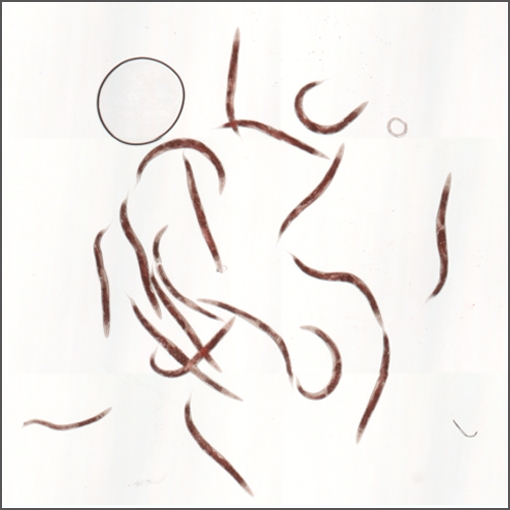
\includegraphics[scale=0.35]{results/test1/original}}
\qquad
  \subfloat[Binary Image]{\label{bin1}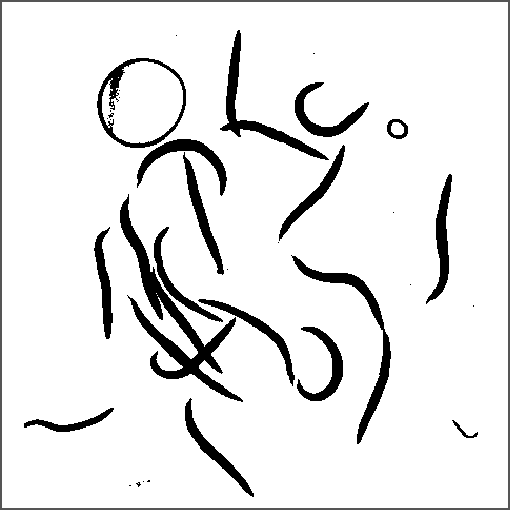
\includegraphics[scale=0.35]{results/test1/binary1}}
\qquad
  \subfloat[Distance map]{\label{dtshape1}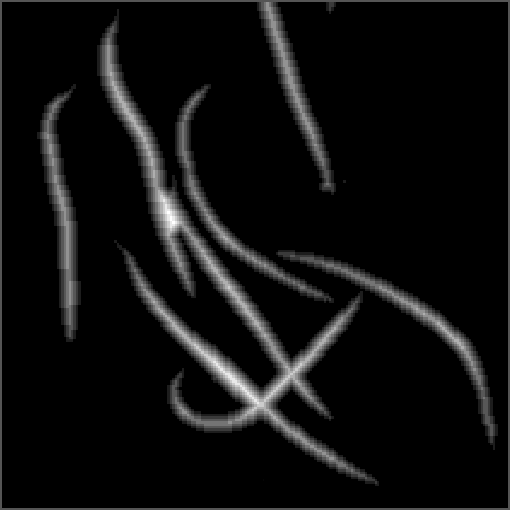
\includegraphics[scale=0.35]{results/test1/dt-shape1}}
\qquad
  \subfloat[Shape skeleton]{\label{skeleton1}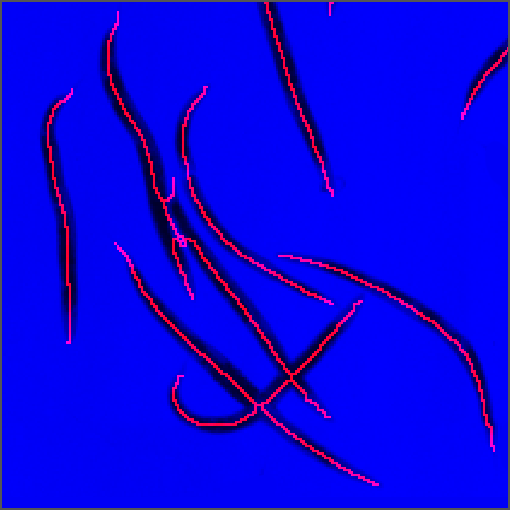
\includegraphics[scale=0.35]{results/test1/sk-full-zoom1}}
\qquad
  \subfloat[Segmentation in Clusters]{\label{clust1}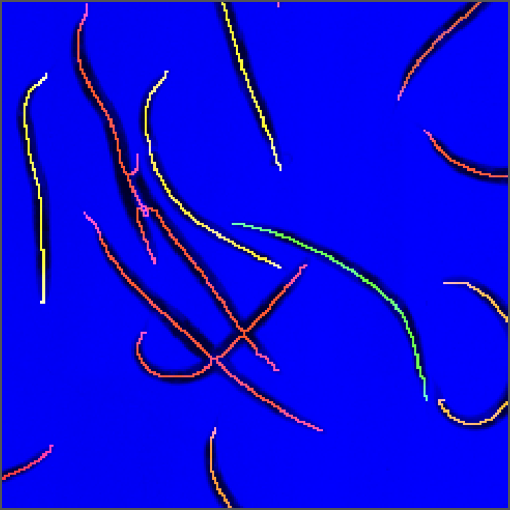
\includegraphics[scale=0.35]{results/test1/cluster-sep1}}
\qquad
  \subfloat[Isolated Worm Profiling]{\label{prof1}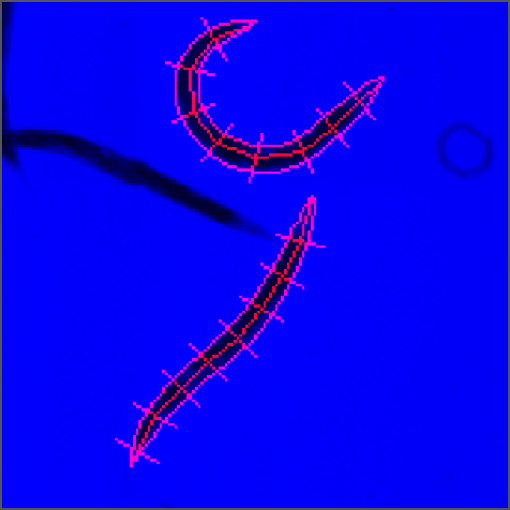
\includegraphics[scale=0.35]{results/test1/profile-zoom}}

  \caption{Sequence of image processing steps before shape matching on test image 1}
\end{figure}

\begin{figure}[h t b p ! H]
  \centering
  \subfloat[Best shape matches]{\label{best1}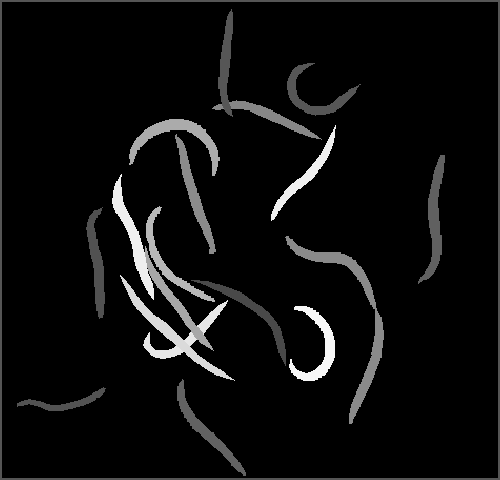
\includegraphics[scale=0.6]{results/test1/complete-frame1}}
\qquad
  \subfloat[Best shape matches over original image]{\label{bestbg1}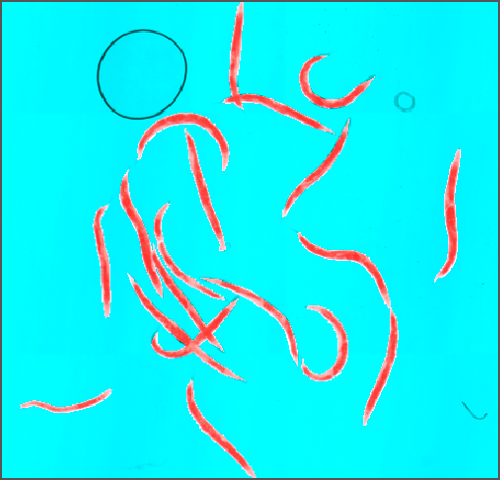
\includegraphics[scale=0.6]{results/test1/complete-framebg1}}
  \caption{Best shape matches on test image 1}
\end{figure}

\begin{figure}[h t b p ! H]
 \centering
   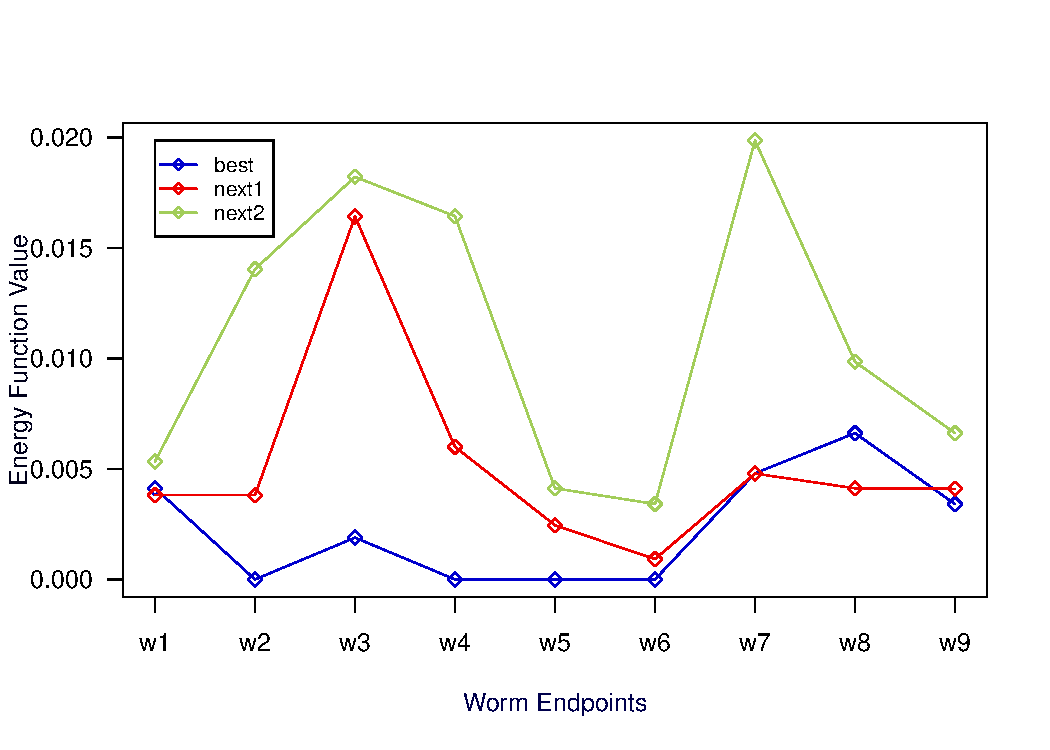
\includegraphics[scale=0.9]{results/test1/energy-graph}
 \caption{Energy value for the best three conformations by endpoint on test
image 1. The selected endpoints correspond to worms in worm clusters that
have more than one possible conformation}
\end{figure}